\chapter{Business logic}

At its most basic form, conferences are meant to be a formal meeting of people with a shared interest, it is meant to be an area where information is exchanged and people get to know each other. Without much thought, we realize that people at conferences are divided into two groups: organizers and visitors; thus, there must be a slight distinction between the two.

% From now on we will refer to organizers as \textbf{admins} and visitors as \textbf{attendees}.

\section{Attendee user flow}

In this subchapter we will analyze what steps an attendee has to go through in order to start using the application, we will start from the very beginning and we will be going into the details of certain features as well as how these can be used. For the purpose of completeness as many steps as possible will be described and images will be used to visualize the said ideas.

\subsection{Visiting the website and signing up}
By visiting the website for the first time we will be greeted with a page where the attendee is prompted to authenticate before using the application.

\begin{figure}[H]
	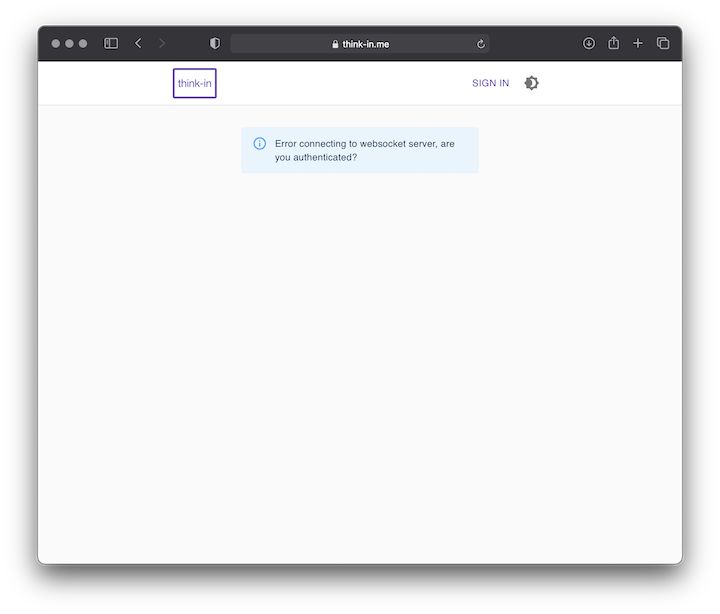
\includegraphics[width=\textwidth,keepaspectratio]{images/business_logic/main_page_not_signed_in.png}
	\caption{Website main page when not signed in.}
	\label{figure:website-main-page}
\end{figure}

An attendee has to have an identity, therefore signing in is necessary before using the application. Upon clicking the \textit{Sign In} button located at the right side of the page header the user is presented with the option of signing in through a third party (social sign in with Google in this case) which significantly speeds up the signing up process, or the more traditional option of using an account created specifically for \textbf{Think-In}.

\begin{figure}[H]
	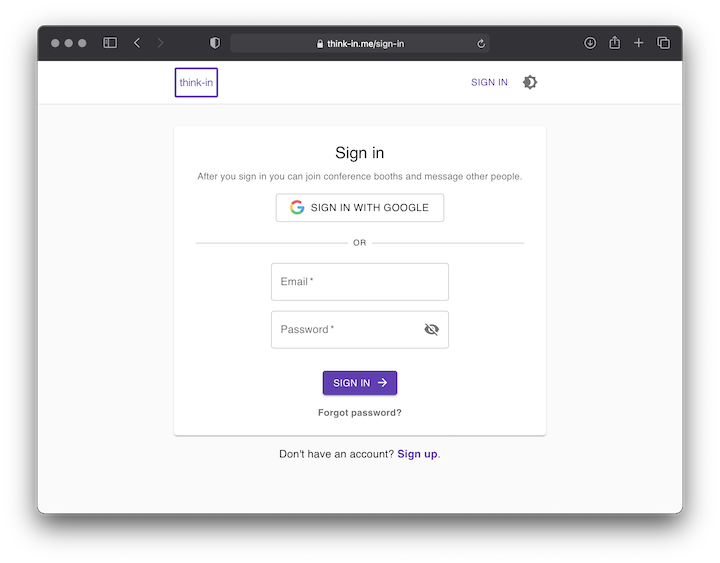
\includegraphics[width=\textwidth,keepaspectratio]{images/business_logic/sign_in_page.png}
	\caption{Website sign in page.}
	\label{figure:website-sign-in-page}
\end{figure}

If the user signs in through an identity provider then he is redirected to the main page (shown in the next subsection), otherwise he has to go to the sign up page by clicking the \textit{Sign Up} button.

\begin{figure}[H]
	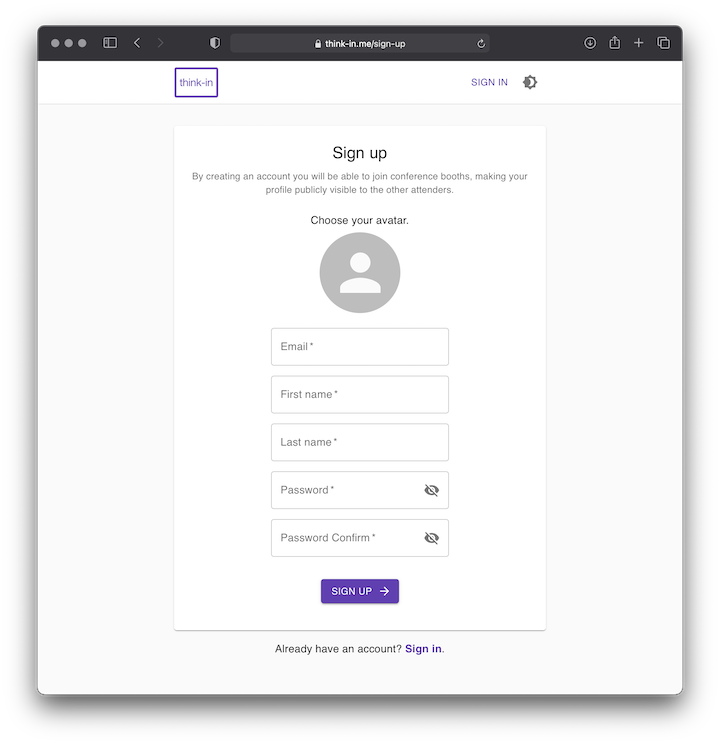
\includegraphics[width=\textwidth,keepaspectratio]{images/business_logic/sign_up_page.png}
	\caption{Website sign up page.}
	\label{figure:website-sign-up-page}
\end{figure}

The user has the choice of selecting an avatar and has to provide the information labeled in the above picture. In case the user did not pick an avatar, an identicon\footnote{\href{https://en.wikipedia.org/wiki/Identicon}{https://en.wikipedia.org/wiki/Identicon}} is generated and is used as the avatar. Upon signing up, the user has to confirm the just created account by following a link sent to the entered email address.

\begin{figure}[H]
	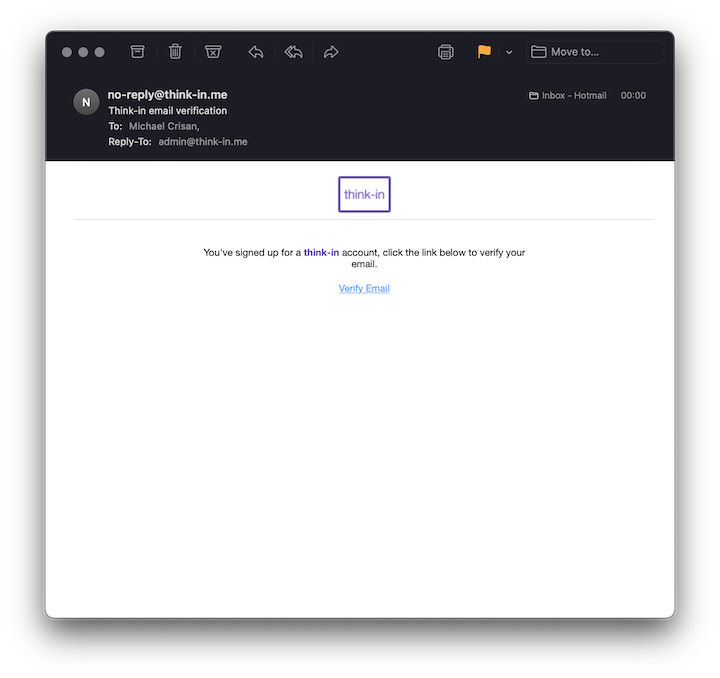
\includegraphics[width=\textwidth,keepaspectratio]{images/business_logic/sign_up_email_confirmation.png}
	\caption{Email confirmation showcasing HTML email.}
	\label{figure:email-confirmation}
\end{figure}

Upon confirming the account and signing in, the user is redirected to the main page.

\subsection{Main page}

The main page is where the users gather and communicate as well as view the media made available by a certain stage.

\begin{figure}[H]
	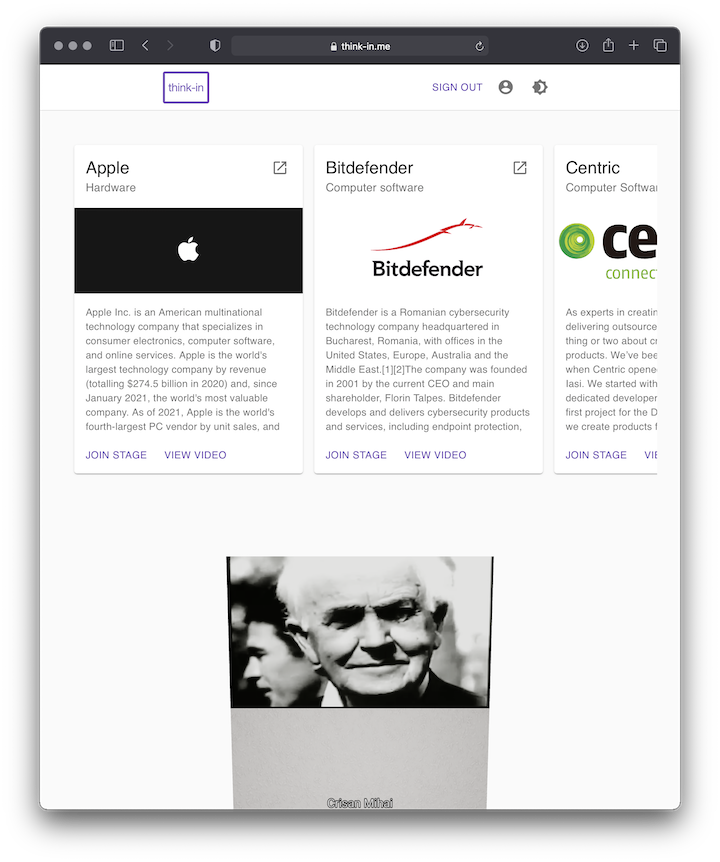
\includegraphics[width=\textwidth,keepaspectratio]{images/business_logic/main_page_signed_in_top.png}
	\caption{Top part of main page when signed in.}
	\label{figure:website-main-page-top}
\end{figure}

In the top part of the main page there is a horizontally scrolling list of stages from which the user can choose to join, every stage has attached a title, subtitle, an external link to the entity representing the stage, a description as well as two actions, \textit{Join Stage} and \textit{View Video}. The first action changes the stage, while the second one gives direct access to the video made available by the entity representing the stage.

\begin{figure}[H]
	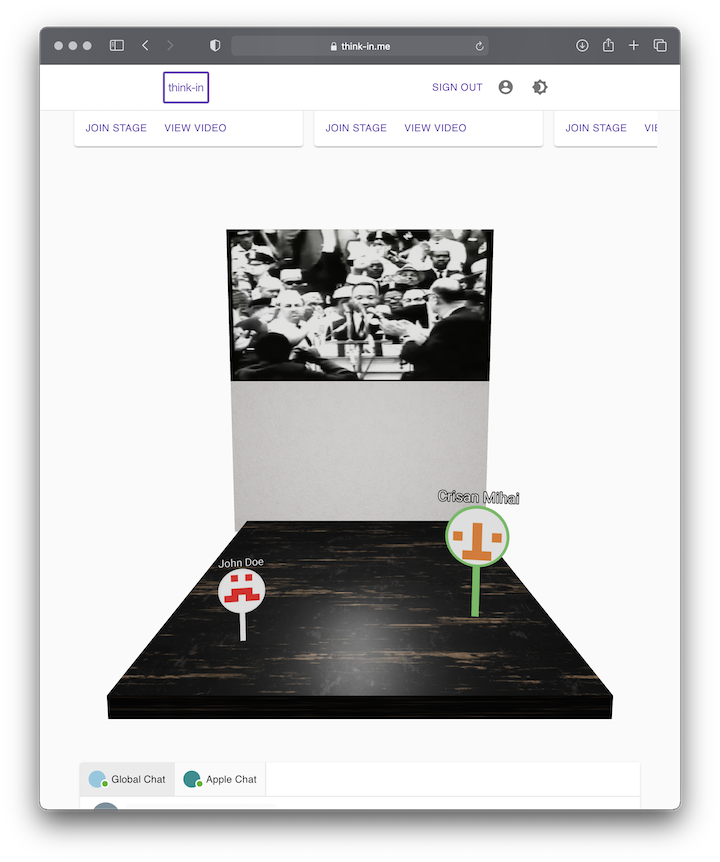
\includegraphics[width=\textwidth,keepaspectratio]{images/business_logic/main_page_signed_in_center.png}
	\caption{Center part of main stage when signed in.}
	\label{figure:website-main-page-center}
\end{figure}

In the center of the main page is the actual stage where users can move their character by simply clicking to the desired location, here the currently present attendees can be seen, in this case \textit{John Doe} and \textit{Crisan Mihai}. As seen in the image above, an attendee is represented by its name and avatar, the current user has a slightly larger character and a green outline instead of grey. The screenshot is taken from the perspective of the user \textit{Crisan Mihai}. In the top part of the stage a looped video is playing, upon clicking it a smooth animation will bring the user closer to the playing media.

\begin{figure}[H]
	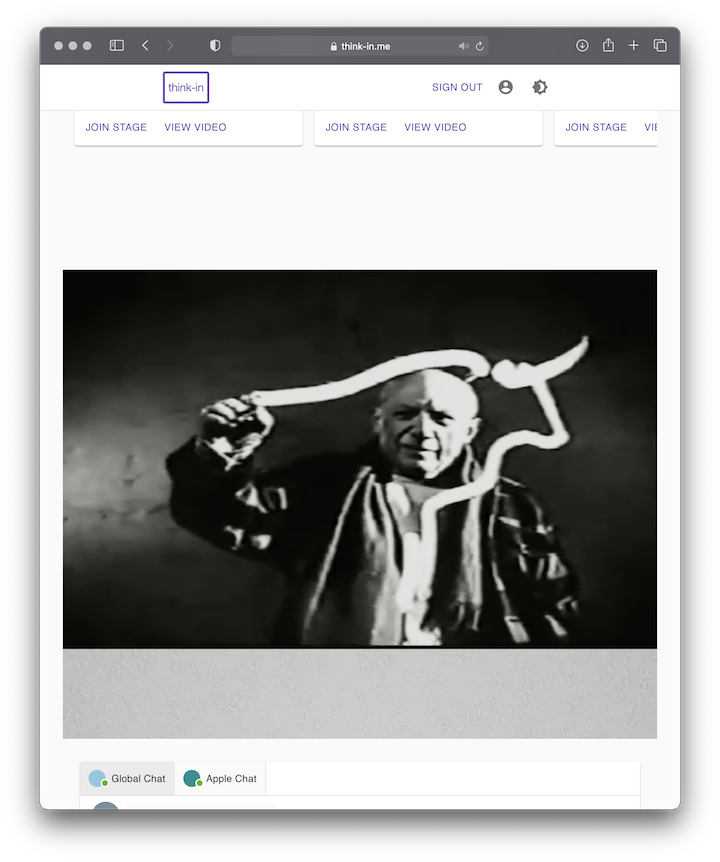
\includegraphics[width=\textwidth,keepaspectratio]{images/business_logic/main_page_signed_in_center_video.png}
	\caption{Media playing in the stage.}
	\label{figure:website-main-page-playing-media}
\end{figure}

When the user doesn't want to see anymore of the video, he simply clicks again on it and is taken back to the default stage view. In the default stage view, the user can click on an attendee's avatar in order to get more information about him.

\begin{figure}[H]
	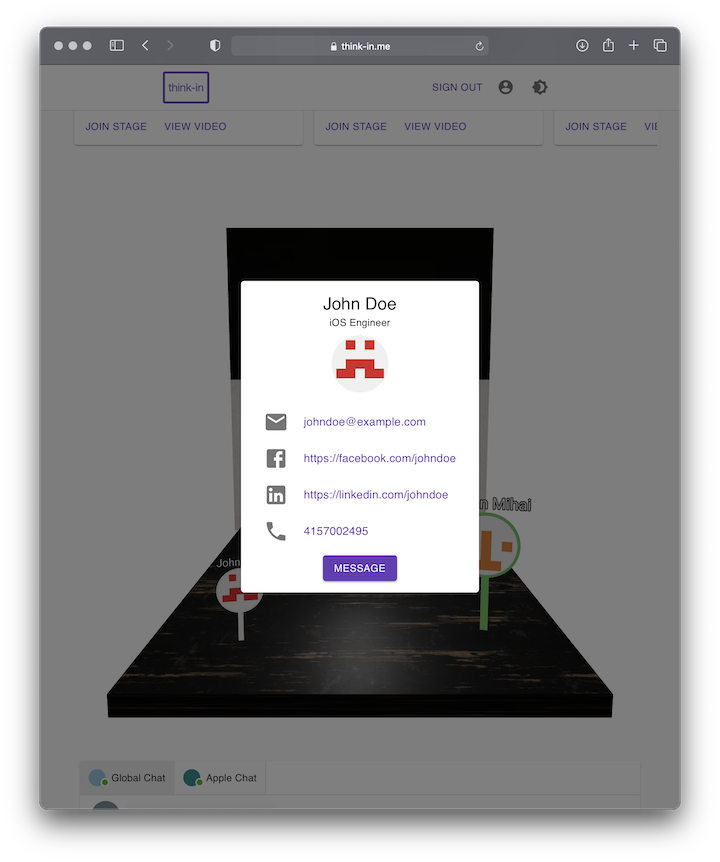
\includegraphics[width=\textwidth,keepaspectratio]{images/business_logic/main_page_signed_in_attendee_dialog.png}
	\caption{Attendee dialog box.}
	\label{figure:website-attendee-dialog-box}
\end{figure}

In the above screenshot we have clicked on \textit{John Doe}'s avatar and a dialog has popped up showing us in addition to his name and avatar which we already knew, his job title (iOS Engineer) and various contact links from where we can gather more information about him. Furthermore, there is a \textit{Message} action that allows us to message \textit{John Doe}, by clicking it a new chat is opened and messages can be sent.

\begin{figure}[H]
	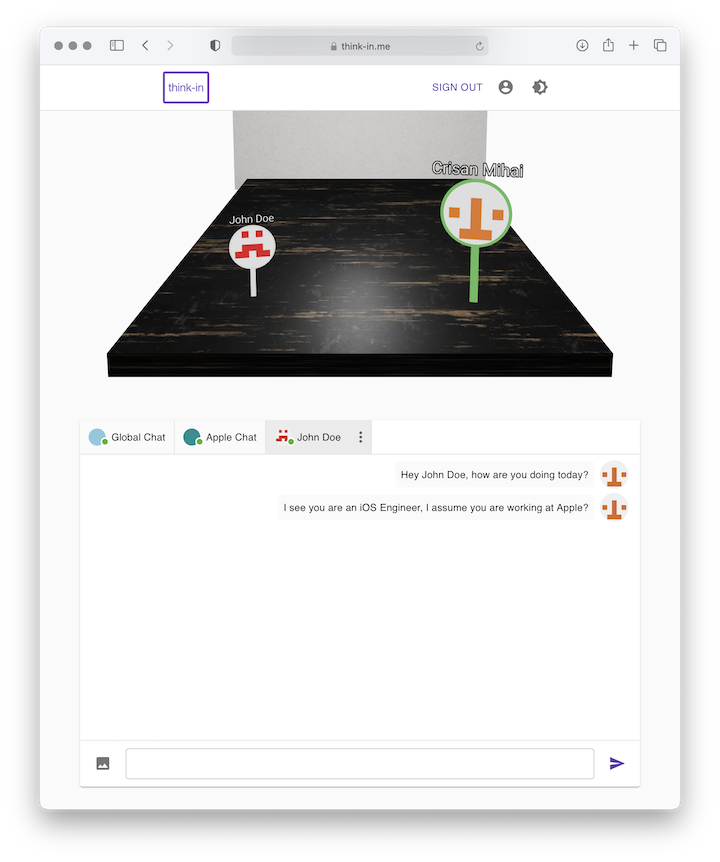
\includegraphics[width=\textwidth,keepaspectratio]{images/business_logic/main_page_signed_in_chat.png}
	\caption{Messaging an attendee, perspective of the sender.}
	\label{figure:website-attendee-messaging-sender}
\end{figure}

The above screenshot is from the perspective of \textit{Crisan Mihai}, what is to be observed is that the messages are translated in your native language, as it is visible in the screenshot below from \textit{John Doe}'s perspective.

\begin{figure}[H]
	\centering
	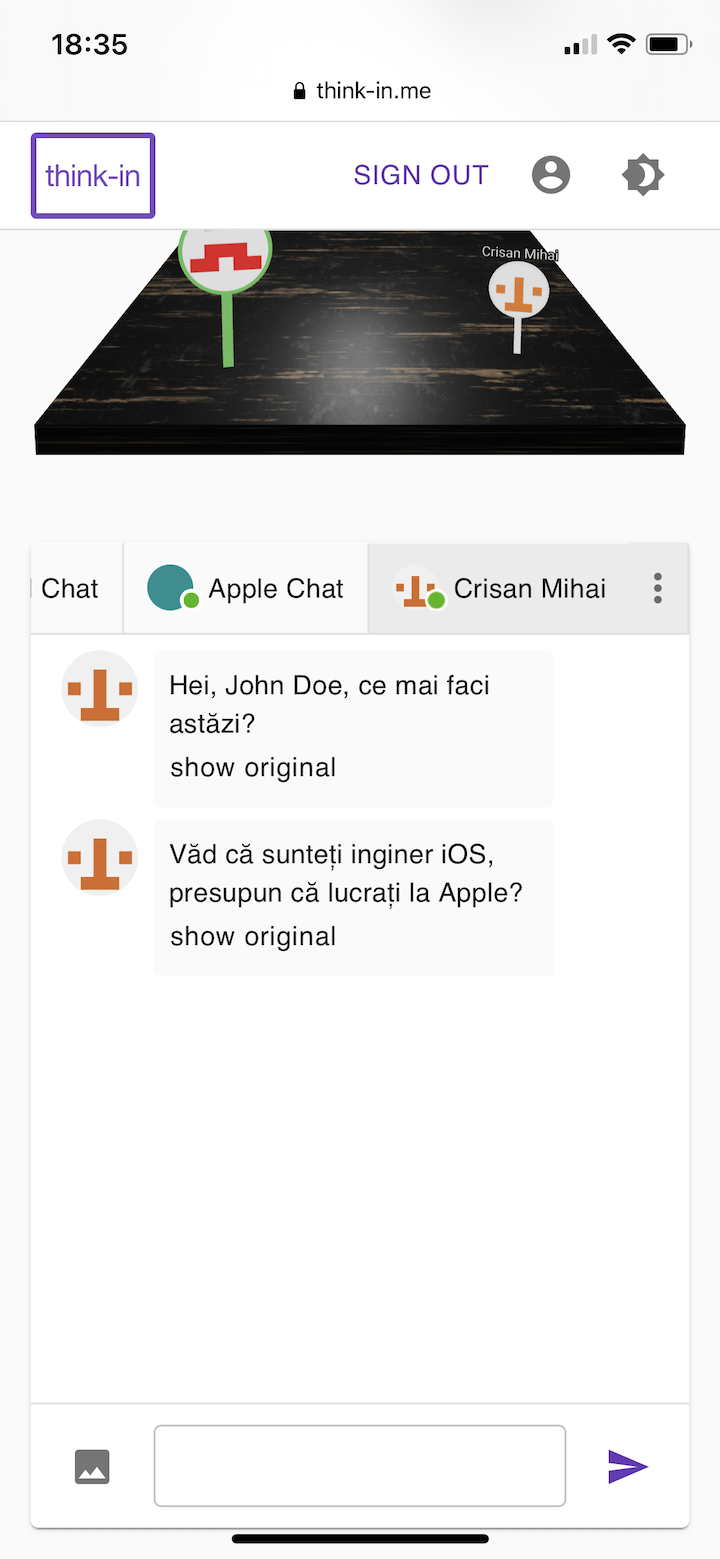
\includegraphics[width=0.5\textwidth,keepaspectratio]{images/business_logic/main_page_signed_in_chat_translated.png}
	\caption{Messaging an attendee, perspective of the receiver which has a different language set than the language of the messages.}
	\label{figure:website-attendee-messaging-receiver}
\end{figure}

Because \textit{John Doe} has selected Romanian as his language, all the messages he sees will be translated into Romanian.

Apart from the just described private chat messages that can be sent only between a pair of users, there are two other types of chats: 
\begin{itemize}
	\item Global chat - in this chat the messages are visible to everyone and it is accessible despite of the selected stage
	\item Stage chat - there is one stage chat for each stage available, i.e. one chat per stage which is only accessible when the user is in that stage
\end{itemize}

\subsection{Profile page}

As shown in the previous subsection, \textit{John Doe} has made available links to his social media but nowhere in the sign up process for instance he was asked to provide this information. There is a page where a user can add data about himself, change the avatar or data he has already provided, the language he speaks in and wants to see the messages in. Furthermore, in this same page a user has the option of changing his email or password as well as deleting his account. A screenshot can be seen below.

\begin{figure}[H]
	\centering
	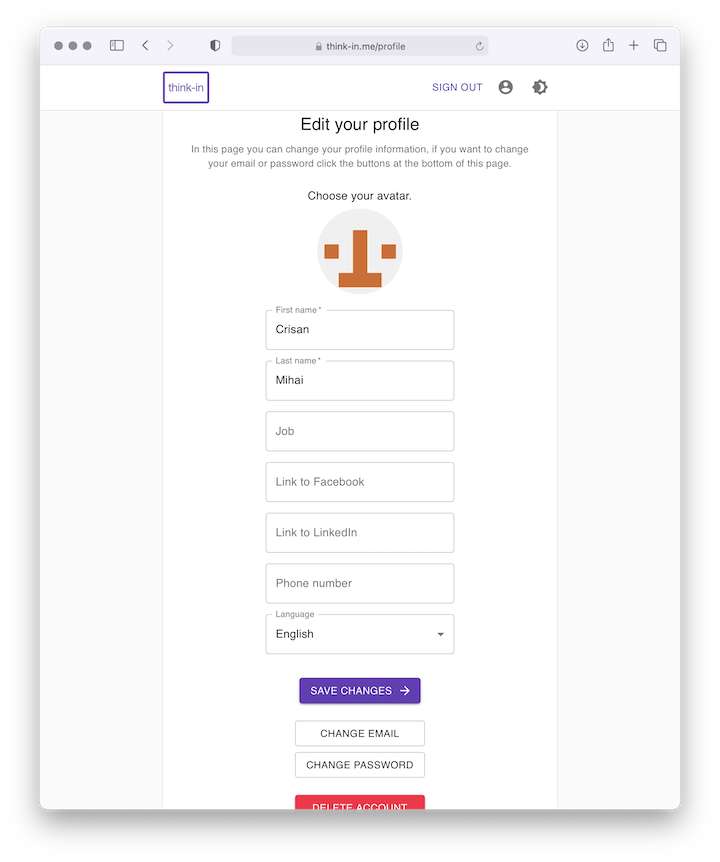
\includegraphics[width=\textwidth,keepaspectratio]{images/business_logic/profile_page.png}
	\caption{Overview of the profile page.}
	\label{figure:website-profile-page}
\end{figure}

It is worth noting that in the case where the user has signed in through a third party, some of the attributes and actions won't be available, to be more explicit the following are not open to change:

\begin{itemize}
	\item Avatar, first name and last name - the data used here are provided by the third party identity provider, if they are to be changed, they have to be changed at the identity provider level
	\item Change email and password actions - there was no email or password set in the first place, therefore there is nothing that can be changed
\end{itemize}

\section{Organizer user flow}

The organizer/admin of the application has the same functionalities as a normal attendee plus the capability of adding, updating or deleting a stage. These functionalities are only visible to organizers/admins and are reachable from the Profile page, which was detailed in the previous section's last subsection. 

The page where a new stage can be added is shown below, media such as image and video can be drag and dropped into the corresponding areas.

\begin{figure}[H]
	\centering
	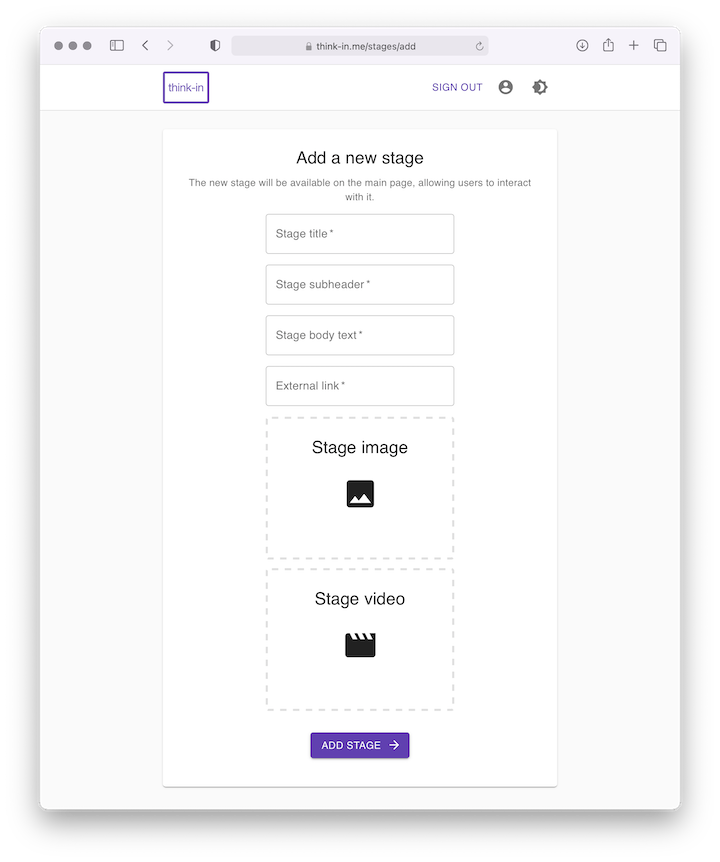
\includegraphics[width=\textwidth,keepaspectratio]{images/business_logic/stages_add.png}
	\caption{Add stage page.}
	\label{figure:add-stage-page}
\end{figure}

The page where a stage can be edited is very similar to the the one where a stage is added, the difference is that the input fields are filled based on the stage selected for editing. What's more is a delete stage action which is self-explanatory.

\begin{figure}[H]
	\centering
	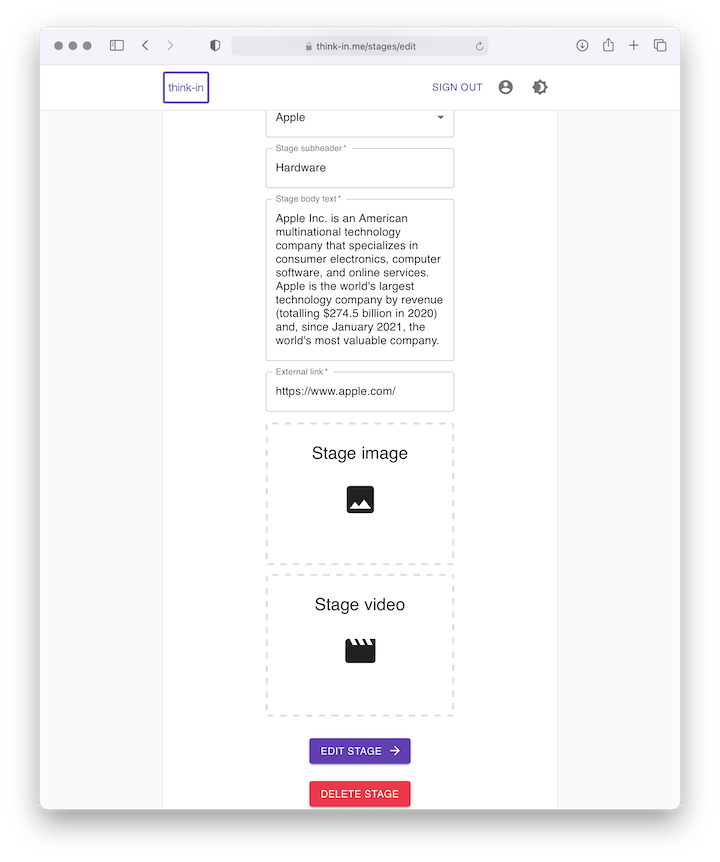
\includegraphics[width=\textwidth,keepaspectratio]{images/business_logic/stages_edit.png}
	\caption{Edit stage page.}
	\label{figure:edit-stage-page}
\end{figure}
